\documentclass[11pt]{article}

% Change "review" to "final" to generate the final (sometimes called camera-ready) version.
% Change to "preprint" to generate a non-anonymous version with page numbers.
\usepackage[final]{acl}

% Standard package includes
\usepackage{times}
\usepackage{latexsym}

% For proper rendering and hyphenation of words containing Latin characters (including in bib files)
\usepackage[T1]{fontenc}
% For Vietnamese characters
% \usepackage[T5]{fontenc}
% See https://www.latex-project.org/help/documentation/encguide.pdf for other character sets

% This assumes your files are encoded as UTF8
\usepackage[utf8]{inputenc}

% This is not strictly necessary, and may be commented out,
% but it will improve the layout of the manuscript,
% and will typically save some space.
\usepackage{microtype}

% This is also not strictly necessary, and may be commented out.
% However, it will improve the aesthetics of text in
% the typewriter font.
\usepackage{inconsolata}

%Including images in your LaTeX document requires adding
%additional package(s)
\usepackage{graphicx}

% If the title and author information does not fit in the area allocated, uncomment the following
%
%\setlength\titlebox{<dim>}
%
% and set <dim> to something 5cm or larger.


\usepackage{amsmath} % 提供强大的数学排版功能，如 equation* 环境
\usepackage{amssymb} % 提供一些额外的数学符号
\usepackage{booktabs}
\usepackage{multirow}
\usepackage{enumitem}
\usepackage{hyperref}
\usepackage{xurl}
\usepackage{amsthm}
\usepackage{threeparttable}

% 必要的包引用
\usepackage{listings}
\usepackage{xcolor}
\usepackage{array}

\usepackage{fontawesome5}
\usepackage{booktabs}
\usepackage{amssymb}
\usepackage{xcolor}

\definecolor{sepseq_green}{HTML}{0B6E4F} % 深绿色
\definecolor{vanilla_grey}{HTML}{6E6E6E} % 灰色

% listings包配置
\lstset{
    basicstyle=\ttfamily\scriptsize,
    commentstyle=\color{gray},
    keywordstyle=\color{black},
    stringstyle=\color{black},
    numberstyle=\tiny\color{+},
    numbers=left,
    numbersep=5pt,
    frame=single,
    frameround=tttt,
    framesep=10pt,
    xleftmargin=20pt,
    xrightmargin=20pt,
    breaklines=true,
    breakatwhitespace=true,
    tabsize=4,
    showspaces=false,
    showstringspaces=false,
    captionpos=b
}

% JSON语言定义
\lstdefinelanguage{json}{
    string=[s]{"}{"},
    stringstyle=\color{-},
    comment=[l]{//},
    morecomment=[s]{/*}{*/},
    commentstyle=\color{gray}\itshape,
    numbers=left,
    numberstyle=\tiny,
    stepnumber=1,
    numbersep=8pt,
    showstringspaces=false,
    breaklines=true,
    frame=lines,
    backgroundcolor=\color{gray!10},
    literate=
     *{0}{{{\color{+}0}}}{1}
      {1}{{{\color{+}1}}}{1}
      {2}{{{\color{+}2}}}{1}
      {3}{{{\color{+}3}}}{1}
      {4}{{{\color{+}4}}}{1}
      {5}{{{\color{+}5}}}{1}
      {6}{{{\color{+}6}}}{1}
      {7}{{{\color{+}7}}}{1}
      {8}{{{\color{+}8}}}{1}
      {9}{{{\color{+}9}}}{1}
      {:}{{{\color{black}{:}}}}{1}
      {,}{{{\color{black}{,}}}}{1}
      {\{}{{{\color{black}{\{}}}}{1}
      {\}}{{{\color{black}{\}}}}}{1}
      {[}{{{\color{black}{[}}}}{1}
      {]}{{{\color{black}{]}}}}{1},
}

\newcommand{\ie}{\emph{i.e., }}
\newcommand{\eg}{\emph{e.g., }}
\newcommand{\etal}{\emph{et al. }}
\newcommand{\st}{\emph{s.t. }}
\newcommand{\etc}{\emph{etc.}}
\newcommand{\wrt}{\emph{w.r.t. }}
\newcommand{\cf}{\emph{cf. }}
\newcommand{\aka}{\emph{a.k.a. }}

\newcommand{\sj}[1]{{\color{black}#1}}
\newcommand{\reversion}[1]{{\color{blue}#1}}
\newcommand{\todo}[1]{{\color{red}#1}}

\newcommand{\cmark}{\textcolor{teal}{\checkmark}}
\newcommand{\xmark}{\textcolor{red!70!black}{\ensuremath{\times}}}
\newcommand{\pmark}{\textcolor{orange!90!black}{\ensuremath{\circ}}}

\newcommand{\spc}{\texttt{\textvisiblespace}}

\definecolor{+}{RGB}{0,128,0} 
\definecolor{-}{RGB}{139,0,0}

\newtheorem{theorem}{Theorem}
\newtheorem{assumption}[theorem]{Assumption}


\title{EasyOPD: An Easy-to-use On-Policy Distillation Framework \\ for Large Language Models}

\author{
    Jie Sun$^{1,3,*,\S}$,
    Mao Zheng$^{2,*}$,
    Mingyang Song$^{2,*}$, 
    Qiyong Zhong$^{1,*,\S}$ \\
    \textbf{Gengsheng Li$^{1,*,\S}$,
    Zhepei Hong$^1$,
    Chang Wu$^1$,
    Pengfei Liu$^3$} \\
    \textbf{Junfeng Fang$^{4,\dagger}$,
    Xiang Wang$^{1,\dagger}$} \\
    $^1$ University of Science and Technology of China \quad $^2$ LLM Department, Tencent \\
    $^3$ Shanghai Innovation Institute \quad $^4$ National University of Singapore \\
    \faGithub\ \href{https://github.com/lds-ustc/EasyOPD}{\textcolor[rgb]{0.0,0.1,0.6}{\texttt{https://github.com/lds-ustc/EasyOPD}}}
}

\begin{document}
\maketitle

\begingroup
\renewcommand{\thefootnote}{}
\footnotetext{
$^{*}$\,Equal Contribution.\quad
$^{\dagger}$\,Corresponding Authors.\quad
$^{\S}$\,Work done during internship at Tencent.}
\endgroup

\begin{abstract}
% 离线蒸馏依赖固定的 teacher 数据，无法覆盖 evolving student 遇到的状态
Conventional language-model distillation often relies on fixed teacher-generated data, which may not cover the states encountered by an evolving student policy.
% OPD 在 student 生成的 rollout 上收集 teacher/evaluator 监督
On-policy distillation (OPD) instead collects teacher or evaluator supervision on student-generated rollouts.
% 现有 OPD 方法在监督形式、tokenizer 兼容性、teacher 访问和监督粒度上差异很大，导致碎片化实现
However, existing OPD methods differ substantially in supervision form, tokenizer compatibility, teacher access, and supervision granularity, leading to fragmented implementations that are difficult to reproduce and extend.
% 提出 EasyOPD，构建在 verl 之上
We present \textsc{EasyOPD}, an on-policy distillation framework built on verl, a distributed reinforcement-learning framework for large language models.
% 分离 user 配置、method 监督逻辑和 verl 执行
\textsc{EasyOPD} separates user-side configuration, method-specific supervision logic, and verl-based execution.
% method module 通过扩展边界连接共享后端
Its method modules connect to the shared backend through extension boundaries for loss construction, rollout metadata, reward processing, tokenizer alignment, and teacher-side computation.
% 实现覆盖四类 OPD 的代表性方法
We implement representative methods covering logit-based OPD, cross-tokenizer OPD, on-policy self-distillation, and step-wise OPD.
% 实验表明这些实现可在同一 verl 后端执行，同时保留各自的目标和性能特征
Experiments on reasoning, code-generation, scientific-knowledge, and tool-use benchmarks show that these implementations can be executed through the same verl-based backend while retaining their method-specific objectives and task-dependent performance profiles.
% 发布代码、配置、文档、demo 包和视频
We release \textsc{EasyOPD} with runnable YAML configurations, documentation, an installable demonstration package, and a demonstration video.

\end{abstract}

% 关于intro的逻辑，我的一个八股文的经验写法（虽然老套，但是有用）：
% 第1段. 首先说自己的task是什么(如sequential rec、explainability、dro)，为什么重要（1-2句话)；然后引出related work，最好以上帝视角来总结related work的common paradigm，不是一个个简单工作的罗列；

% 第2段. 指出现有paradigm的limitation，必须佐以intuitive example/experiments + teaser figure；

% 第3段. 介绍key idea，注意是从idea层面来如何解决这个limitation的，结合第二段中的example和figure；

% 第4段. 介绍key tech，注意是从technical层面来介绍如何实现key idea的，最好以庖丁解牛的思维来写：分不同模块，每个模块核心tech是啥，为啥能解决limitation；

% 第5段. 介绍效果；

\section{Introduction}

Large language model distillation transfers capabilities from a stronger teacher to a smaller, more efficient student, aiming to reduce deployment costs while retaining reasoning, coding, and instruction-following abilities~\citep{alkhulaifi2021knowledge_kd}.
Conventional distillation uses teacher responses or token distributions on fixed contexts~\citep{yang2024kd_survey}.
At inference, however, the student conditions on its own prefixes and may encounter contexts poorly covered by offline supervision~\citep{gu2024minillm_opd,ko2024distillm_opd}.
On-policy distillation (OPD) mitigates this mismatch through a common loop: the current student generates rollouts, a teacher or evaluator supervises them, and the resulting signals guide student updates~\citep{song2026survey,lu2025onpolicydistillation}.
OPD methods vary by supervision interface, tokenizer compatibility, and granularity, with overlapping settings including logit-based distillation, cross-tokenizer alignment, self-OPD, black-box or rubric-based feedback, and step-wise or agentic supervision.


\begin{figure*}[t]
    \centering
    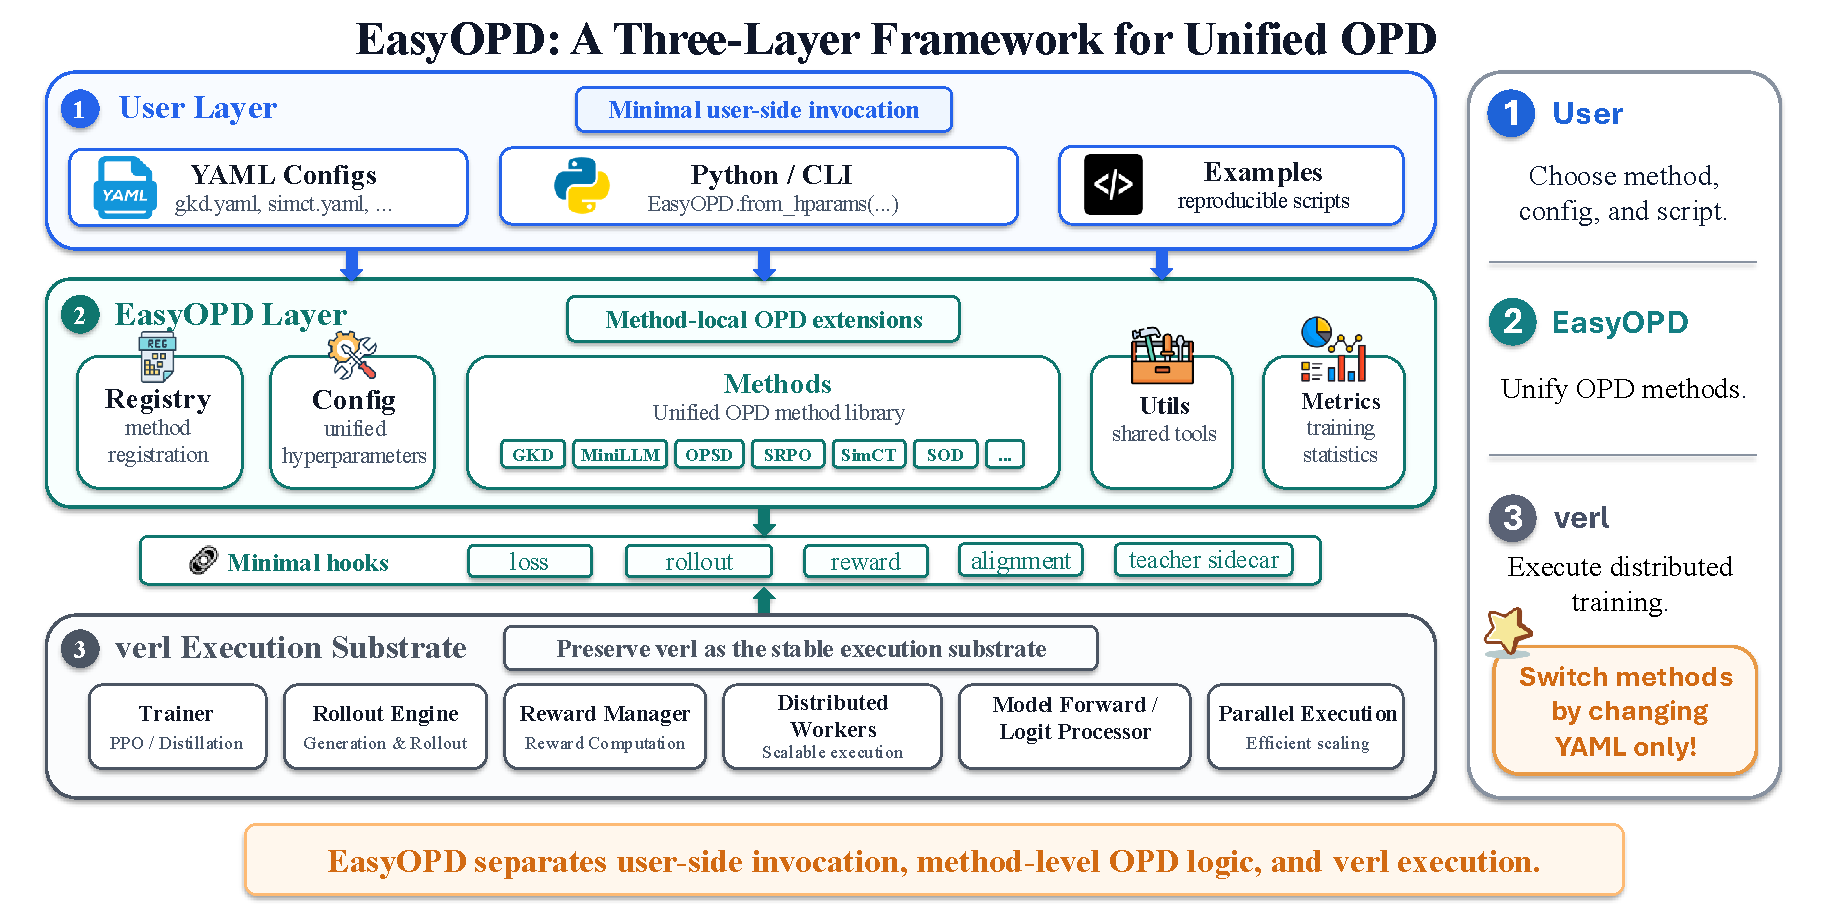
\includegraphics[width=1.0\textwidth]{figures/framework_0526.pdf}
    \caption{Architecture of \textsc{EasyOPD}. The user layer provides configuration-based invocation, the \textsc{EasyOPD} layer encapsulates method-local OPD logic, and verl provides distributed execution. Hooks for loss, rollout, reward, alignment, and teacher-side computation connect method modules to verl, allowing supported methods to share the same execution backend and be selected via YAML configurations.}
    \label{fig:framework}
\end{figure*}


A shared algorithmic paradigm does not yield a common system interface.
Depending on the supervision, OPD may span rollout generation, teacher inference, cross-tokenizer alignment, reward construction, distributed data flow, and optimization.
For example, cross-tokenizer OPD requires alignment or projection across teacher and student tokenizations before constructing compatible supervision, whereas black-box or rubric-based OPD may convert textual judgments or scores from a teacher or evaluator into rewards or training objectives; these supervision patterns therefore require different extension points.
Existing frameworks address complementary parts of the OPD workflow: TRL~\citep{vonwerra2020trl} provides trainer-centric distillation APIs; verl~\citep{sheng2024hybridflow_verl} and slime~\citep{slime_github} support scalable on-policy rollout and distributed execution; and KDFlow~\citep{zhang2026kdflow} provides a distillation-oriented stack.
However, as summarized in Table~\ref{tab:opd-frameworks}, we find no single reviewed framework that documents method-local extension boundaries across the heterogeneous supervision interfaces considered in this work while reusing a common distributed backend.
This gap calls for a lightweight OPD abstraction linking method-specific supervision to a shared execution substrate.


To fill this gap, we present \textsc{EasyOPD}, a unified OPD framework built on verl.
\textsc{EasyOPD} reuses verl for rollout generation, model execution, and optimization while adding a lightweight abstraction layer for method-local supervision.
Method modules connect to the shared training flow through explicit extension points: cross-tokenizer methods localize alignment and supervision construction, whereas black-box or rubric-based methods localize feedback acquisition and training-signal construction.
This design turns OPD integration from framework-wide modification into method-local extension.


To realize this design, \textsc{EasyOPD} adopts the three-layer architecture shown in Figure~\ref{fig:framework}. 
The user layer provides Python and CLI entry points and YAML configurations for specifying methods, teacher and student models, datasets, and hyperparameters.
The \textsc{EasyOPD} layer manages method registration, method-local modules, shared utilities, and supervision diagnostics.
Each module handles supervision acquisition, transformation, use, and diagnostics, and connects to verl through dispatch hooks for loss, rollout metadata, reward, alignment, and teacher-side computation.
The verl layer handles distributed rollout, model execution, worker orchestration, reward computation, and optimization.
Users select supported methods through configuration, while developers add methods by implementing and registering modules with the required hooks. For the evaluated implementations, method-specific supervision logic is placed in registered method-local modules, and the core trainer and workers interact with them only through the shared dispatch layer.
Through these layers, we implement and evaluate representative methods across three settings: cross-tokenizer OPD, on-policy self-distillation, and step-wise OPD. The framework also implements logit-based OPD, and its extension boundaries are designed to accommodate additional supervision forms such as black-box or rubric-based feedback.


We evaluate \textsc{EasyOPD} through three case studies covering cross-tokenizer OPD, on-policy self-distillation, and step-wise OPD.
Within each setting, methods share the model initialization, training data, execution backend, and evaluation procedure where applicable, while retaining their original supervision designs.
Once the shared hook layer is in place, each evaluated method concentrates its supervision logic in a small set of registered method-local files and reuses the existing dispatch sites in the core rather than introducing new method-specific components; we report the per-method integration cost in Section~\ref{sec:experiments}.
We further report framework overhead relative to matched verl runs in Section~\ref{sec:experiments}, separating teacher-inference, alignment, and reward-evaluation costs from the dispatch layer itself.
We release the code under the Apache License 2.0 on GitHub with reproducible YAML configurations, documentation, and an installable demonstration package with runnable examples.

\section{Background and Motivation}

\paragraph{Previous Solutions.}
Knowledge distillation (KD) typically trains a smaller student model to imitate the predictive behavior of a larger or more capable teacher~\citep{hinton2015distilling_kd,ko2024distillm_opd}. For autoregressive language models, common offline approaches include sequence-level distillation, in which the student is trained on teacher-generated sequences~\citep{kim2016sequence}, and supervised token-level KD, in which the student matches the teacher's next-token distributions along prefixes induced by a fixed offline set of output sequences~\citep{agarwal2024onpolicy_opsd}. These output sequences may be ground-truth or teacher-generated. In their purely offline form, both approaches optimize over an output-prefix distribution that does not track the current student's rollout distribution. During autoregressive inference, however, the student conditions on its own previous predictions. A deviation can therefore shift subsequent prefixes away from those observed during offline distillation, creating a training--inference distribution mismatch and allowing errors to compound across decoding steps~\citep{lin2020imitkd,agarwal2024onpolicy_opsd}.


\paragraph{On-Policy Distillation Mechanism.}
On-policy distillation (OPD) collects teacher supervision on outputs generated by the current student, rather than relying only on fixed offline sequences. During training, the student generates responses or trajectories, and the teacher provides supervision on the resulting prefixes or states. The student is then updated, and new rollouts are generated with the updated policy. In a common white-box setting, the teacher provides next-token distributions on student-generated prefixes, and the student minimizes a token-level divergence from the teacher~\citep{agarwal2024onpolicy_opsd}. The defining property of OPD is therefore that supervision is collected on states induced by the current student, rather than the use of any particular distillation objective~\citep{lu2025onpolicydistillation,song2026survey}.

Training on student-generated states helps reduce the mismatch between offline training data and the prefixes encountered during autoregressive inference, while providing guidance on errors made by the student itself~\citep{agarwal2024onpolicy_opsd,ko2024distillm_opd}. However, OPD also turns distillation into an iterative pipeline that must coordinate student rollout, teacher inference, supervision construction, and model optimization. Since OPD methods differ in teacher access, feedback form, and training objectives~\citep{song2026survey}, a practical framework should support this shared pipeline while allowing method-specific supervision to be implemented consistently.

\section{Design and Implementation}

\begin{table*}[t]
\centering
\small
\caption{
Comparison of OPD supervision interfaces and framework properties.
\cmark\ denotes native or first-class support, \pmark\ denotes partial
or experimental support, and \xmark\ denotes no documented support.
\emph{On-policy self-distillation} refers to settings in which the
teacher is derived from the student model and supervises
student-generated rollouts. The comparison reflects publicly documented
functionality as of July 2026, using the versions or commits
listed in Appendix~\ref{app:framework-comparison}, where per-cell evidence
is also provided.
}
\setlength{\tabcolsep}{6pt}
\begin{tabular}{l cccc ccc}
\toprule
 & \multicolumn{4}{c}{\textbf{OPD supervision-interface coverage}}
 & \multicolumn{3}{c}{\textbf{Framework properties}} \\
\cmidrule(lr){2-5}\cmidrule(lr){6-8}

\textbf{Framework}
 & \shortstack{Logit\\OPD}
 & \shortstack{Cross-tok.\\OPD}
 & \shortstack{On-policy\\self-distill.}
 & \shortstack{Step-wise\\OPD}
 & \shortstack{Released\\YAML/CLI}
 & \shortstack{Documented method\\extension API}
 & \shortstack{Compatible w/\\multi-node} \\
\midrule

TRL
 & \cmark
 & \pmark
 & \pmark
 & \xmark
 & \cmark
 & \xmark
 & \pmark \\

verl
 & \cmark
 & \xmark
 & \xmark
 & \pmark
 & \cmark
 & \xmark
 & \cmark \\

slime
 & \cmark
 & \xmark
 & \pmark
 & \pmark
 & \cmark
 & \xmark
 & \cmark \\

KDFlow
 & \cmark
 & \cmark
 & \cmark
 & \xmark
 & \cmark
 & \pmark
 & \pmark \\

\textbf{Ours}
 & \cmark
 & \cmark
 & \cmark
 & \cmark
 & \cmark
 & \cmark
 & \cmark\,{\footnotesize(via verl)} \\

\bottomrule
\end{tabular}

\label{tab:opd-frameworks}
\end{table*}

% Figure 2: EasyOPD running example (SimCT). All field names, the launch
% command, and the diagnostic metric names are copied from the released
% repository (easyopd/config/simct.yaml, examples/simct/run_simct.sh, and
% easyopd/methods/simct/losses.py).
\begin{figure*}[t]
    \centering
    \footnotesize
    \setlength{\fboxsep}{4pt}
    %---------------- Left: YAML + CLI ----------------%
    \begin{minipage}[t]{0.31\textwidth}
        \raggedright
        \textbf{(a) Declarative configuration}\\[2pt]
        \begin{lstlisting}[basicstyle=\ttfamily\tiny,frame=single,numbers=none,language=]
# config/simct.yaml
student_model_path: Qwen/Qwen3-8B
teacher_model_path:
  meta-llama/Llama-3.2-3B-Instruct
distillation:
  enabled: true
  distillation_loss:
    loss_mode: simct
    cross_tokenizer_kl_direction:
      reverse
    use_task_rewards: false
        \end{lstlisting}
        \textbf{Launch}\\[2pt]
        \begin{lstlisting}[basicstyle=\ttfamily\tiny,frame=single,numbers=none,language=bash]
bash examples/simct/run_simct.sh
        \end{lstlisting}
    \end{minipage}
    \hfill
    %---------------- Middle: dispatch ----------------%
    \begin{minipage}[t]{0.32\textwidth}
        \raggedright
        \textbf{(b) Resolution and hook composition}\\[6pt]
        \fbox{\parbox{0.92\linewidth}{\centering Config}}\\[2pt]
        \centering$\downarrow$\\[2pt]
        \fbox{\parbox{0.92\linewidth}{\centering Registry (\texttt{loss\_mode=simct})}}\\[2pt]
        $\downarrow$\\[2pt]
        \fbox{\parbox{0.92\linewidth}{\centering SimCT module:\\ cross-tokenizer alignment\\ +\ teacher sidecar\ +\ loss}}\\[2pt]
        $\downarrow$\\[2pt]
        \fbox{\parbox{0.92\linewidth}{\centering verl: rollout + optimization}}\\[6pt]
        \raggedright Only the hooks required by SimCT are activated; other methods activate a different subset.
    \end{minipage}
    \hfill
    %---------------- Right: diagnostics ----------------%
    \begin{minipage}[t]{0.31\textwidth}
        \raggedright
        \textbf{(c) Supervision diagnostics}\\[2pt]
        \begin{lstlisting}[basicstyle=\ttfamily\tiny,frame=single,numbers=none,language=]
distillation/overlap_vocab_size
distillation/simct_valid_segments
distillation/simct_span_segments
distillation/simct_skipped_samples
distillation/simct_valid_span_ratio
distillation/simct_loss
        \end{lstlisting}
        \raggedright In addition to task performance, EasyOPD logs whether the intended cross-tokenizer supervision is active.
    \end{minipage}
    \caption{A running example of launching SimCT with \textsc{EasyOPD}. The YAML configuration selects the method and resolves its method-specific options; the registry activates the required alignment, teacher-side, and loss hooks; verl executes rollout generation and optimization, while \textsc{EasyOPD} reports supervision-specific diagnostics. Field names, the launch command, and the diagnostic metric names are taken from the released repository.}
    \label{fig:running_example}
\end{figure*}


EasyOPD provides a unified OPD training process on top of verl. Instead of treating each OPD method as an isolated training script, it decomposes an OPD run into four reusable stages: method invocation, configuration resolution, supervision construction, and distributed execution. This section describes how these stages form a unified workflow that connects diverse OPD methods to the same verl execution substrate.

\subsection{A Unified OPD Workflow}

Although OPD methods differ in their supervision interfaces, they share a common training flow. Given a teacher model, a student model, and training data, the student first generates on-policy rollouts; the selected method then constructs supervision on these rollouts, such as teacher logits, aligned token distributions, judge rewards, or step-level feedback; finally, the training system consumes this supervision through loss computation, reward aggregation, or trajectory-level weighting. EasyOPD makes this shared process explicit and standardizes invocation and dispatch, without requiring all methods to share a single loss, teacher interface, or evaluation metric. As shown in Figure~\ref{fig:framework}, the user layer specifies what to run, the EasyOPD layer defines how supervision is constructed, and the verl layer executes the resulting training process on top of its distributed runtime~\citep{sheng2024hybridflow_verl}.

\subsection{Declarative Invocation and Configuration}

EasyOPD exposes OPD methods through declarative configurations and launch scripts. Released methods can be selected through method-specific YAML configurations without manually editing rollout workers, reward managers, logit processors, or trainer-side loss assembly, which turns method selection into a configuration-level operation and makes experiments easier to reproduce. Figure~\ref{fig:running_example} shows a concrete running example in which the same \texttt{from\_hparams} entry point and a single launch command drive all three studied settings---cross-tokenizer OPD, on-policy self-distillation, and step-wise OPD---together with their baselines, changing only the method name and its YAML configuration.

Different OPD methods require different options: logit-based methods may specify divergence directions or top-$k$ support; cross-tokenizer methods may specify alignment or overlap-vocabulary behavior; rubric-based methods may specify judge prompts or reward aggregation rules; step-wise methods may specify trajectory segmentation or weighting strategies. EasyOPD keeps these choices in a unified configuration space and resolves them through method registration, so new methods can be added without hard-coding method choices into the trainer.

\subsection{Method-Local Supervision Logic}

The core of EasyOPD is to localize OPD-specific supervision logic: a method defines how supervision is obtained, transformed, consumed, and diagnosed. Standard OPD may only require a token-level distillation objective, cross-tokenizer OPD may require tokenizer or span alignment and a common supervision space, rubric-based OPD may convert judge feedback into rewards, and step-wise OPD may attach feedback to intermediate reasoning states or multi-turn trajectories. EasyOPD does not force these methods into a single loss-only abstraction; it gives each a local space to implement the supervision interface it needs.

Method-local logic also includes diagnostics. Implemented method modules expose supervision-specific diagnostics in addition to task performance, so users can check whether the intended supervision signal is active, not only the final loss. For example, the released cross-tokenizer implementation reports the overlap-vocabulary size, the number of valid and span-level aligned segments, the count of skipped samples, and the valid-span ratio, while the step-wise implementation reports the mean step-level weight and the number of supervised steps. These metrics help users debug failures that final task performance alone cannot explain.

\subsection{Execution through Thin verl Hooks}

EasyOPD reuses verl as the execution substrate instead of reimplementing distributed training. verl provides the system-heavy components required by OPD, including rollout generation, reward computation, model forwarding, logit processing, distributed workers, trainer-side optimization, and parallel execution, and EasyOPD connects method-local supervision logic to this substrate through a small set of thin hooks.

A hook is a dispatch boundary rather than a method implementation: it exposes a stable interaction point in the training pipeline and routes the corresponding data or control flow to the selected method module. The hook set covers the main entry points of OPD supervision: loss hooks for token- or distribution-level supervision, rollout hooks for trajectory metadata, reward hooks for judge or rubric feedback, alignment hooks for token- or span-level mapping, and teacher-sidecar hooks for teacher-side signals such as logits, hidden states, or judge outputs, as used respectively by logit-based, feature-based~\citep{zhang2024dskd}, and rubric-based methods.

This design balances expressiveness and maintainability. Writing every method directly into verl would create method-specific branches, while exposing only a single fixed interface would make alignment-, reward-, or trajectory-based OPD methods difficult to express. Thin hooks keep method logic local while verl remains the shared backend. EasyOPD thus inherits rollout generation, worker orchestration, optimization, and distributed execution from verl; its contribution is the dispatch layer connecting these components to method-local supervision logic.

\section{Experiments}
\label{sec:experiments}


\subsection{Experimental Setup}
\label{sec:exp_setup}

We evaluate \textsc{EasyOPD} in three settings that exercise different method-specific interfaces. Cross-tokenizer OPD requires supervision across different teacher and student tokenizations. On-policy self-distillation instantiates teacher and student policies from the same model under different conditioning contexts. Step-wise OPD assigns supervision to intermediate reasoning or tool-interaction steps. These settings cover variation in supervision space, teacher conditioning, and supervision granularity, and are not intended as a single cross-regime leaderboard.

\paragraph{Cross-tokenizer OPD.}
Standard OPD directly compares teacher and student next-token distributions, which are not naturally aligned under different tokenizers; cross-tokenizer methods address this by constructing a shared supervision space. We compare SimCT \citep{sun2026simctrecoveringlostsupervision}, ULD \citep{boizard2025uld}, ALM \citep{minixhofer2025alm}, and DSKD \citep{zhang2024dskd}, distilling Qwen2.5-7B-Instruct \citep{qwen25} into Phi-4-mini-Instruct \citep{phi4mini}. All methods start from the same student checkpoint, warm-started on a shared 10K teacher-generated math and code corpus, and use the same training prompts and optimization budget. We evaluate on MATH500 \citep{lightman2023math500}, GSM8K~\citep{cobbe2021training_gms8k}, MBPP~\citep{austin2021program_mbpp}, and LiveCodeBench v6~\citep{jain2024livecodebench}, reporting exact-match accuracy for reasoning and pass@1 for code.

\paragraph{On-policy self-distillation.}
On-policy self-distillation (OPSD) uses the same base model under different conditioning contexts: the student generates a response from the original prompt, while the self-teacher re-evaluates it with additional feedback. We instantiate this setting with SDPO~\citep{hubotter2026sdpo}, using Qwen3-8B~\citep{qwen2025qwen3} as both the student and self-teacher, and compare it with the base model and GRPO~\citep{shao2024deepseekmath}. We evaluate Chemistry from SciKnowEval~\citep{feng2024sciknoweval}, Biology from SciKnowEval~\citep{feng2024sciknoweval}, Tool Use from ToolAlpaca~\citep{tang2023toolalpaca}, and mathematical reasoning on GSM8K~\citep{cobbe2021training_gms8k}. We report the highest Average@16 reached within one-hour and five-hour wall-clock budgets, where Average@16 is the mean correctness over 16 independently sampled responses per question.

\paragraph{Step-wise OPD.}
Response-level OPD~\citep{agarwal2024onpolicy_opsd} applies teacher supervision uniformly across a trajectory, although supervision on later steps may become less reliable after erroneous tool interactions. SOD~\citep{zhong2026sod} instead reweights the distillation loss by step-level student--teacher divergence. We use Qwen3-1.7B~\citep{qwen2025qwen3} as the student and a GRPO-optimized Qwen3-4B~\citep{zhong2026sod} as the teacher, comparing the base model, GRPO~\citep{shao2024deepseekmath}, response-level OPD, and SOD under a shared SFT initialization, training data, and optimization budget \citep{zhong2026sod}. We evaluate on AIME 2024, AIME 2025~\citep{maa_aime}, and LiveCodeBench v6~\citep{jain2024livecodebench}; each score is Average@32 over 32 sampled responses per problem, and Avg.\ is their unweighted mean.

\paragraph{Shared implementation.}
All methods are implemented in \textsc{EasyOPD} and executed through the same verl-based infrastructure~\citep{sheng2024hybridflow_verl}. Within each setting, we keep the model configuration, training data, execution backend, and evaluation procedure fixed where applicable, while retaining each method's original supervision design. Additional optimization, sampling, hardware, and checkpoint details are provided in the Appendix~\ref{app:exp_setup}.


\subsection{Results}
\label{sec:exp_results}

\paragraph{Cross-tokenizer OPD.}
Table~\ref{tab:cross_tokenizer_results} shows that all four evaluated cross-tokenizer methods improve the unweighted average over the base student. SimCT obtains the highest average (53.5, +3.3 over the base) and the best MATH500, ALM leads on MBPP and LiveCodeBench v6, and DSKD is best on GSM8K. This confirms that the evaluated cross-tokenizer objectives run through \textsc{EasyOPD}'s alignment and loss interfaces under a matched setup, while retaining distinct task-dependent profiles.


\begin{table}[t]
    \centering
    \small
    \setlength{\tabcolsep}{4pt}
    \renewcommand{\arraystretch}{1.15}
    \caption{Cross-tokenizer OPD results. Reasoning scores are exact-match accuracy, code scores are pass@1, and Avg.\ is their unweighted mean. Best per column in bold.}
    \label{tab:cross_tokenizer_results}
    \begin{tabular}{lccccc}
        \toprule
        Method
        & MATH500
        & GSM8K
        & MBPP
        & LCB-v6
        & Avg. \\

        \midrule

        Base
        & 54.2
        & 86.0
        & 53.2
        & 7.4
        & 50.2 \\

        \midrule

        ULD
        & 57.0
        & 85.1
        & 55.4
        & 9.1
        & 51.7 \\

        ALM
        & 58.2
        & 84.9
        & \textbf{56.4}
        & \textbf{12.0}
        & 52.9 \\

        DSKD
        & 58.8
        & 86.4
        & 56.2
        & 9.7
        & 52.8 \\

        SimCT
        & \textbf{59.6}
        & \textbf{86.7}
        & \textbf{56.4}
        & 11.4
        & \textbf{53.5} \\

        \bottomrule
    \end{tabular}
\end{table}
\begin{table}[t]
    \centering
    \small
    \setlength{\tabcolsep}{3.5pt}
    \renewcommand{\arraystretch}{1.15}
    \caption{
    SDPO and GRPO in the OPSD setting under one-hour and five-hour wall-clock
budgets. Average@16 is the mean correctness over 16 sampled responses per
question; Base is the untrained checkpoint, reported once per task. We evaluate
every five steps and report the best Average@16 observed within each budget;
the best per task and budget is in bold.
    }
    \label{tab:self_opd_results}
    \begin{tabular}{lcccccccc}
        \toprule
        & \multicolumn{8}{c}{$\mathrm{avg@16}$} \\
        \cmidrule(lr){2-9}
        Method
        & \multicolumn{2}{c}{Chemistry}
        & \multicolumn{2}{c}{Biology}
        & \multicolumn{2}{c}{Tool Use}
        & \multicolumn{2}{c}{GSM8K} \\
        \cmidrule(lr){2-3}
        \cmidrule(lr){4-5}
        \cmidrule(lr){6-7}
        \cmidrule(lr){8-9}
        & 1h & 5h
        & 1h & 5h
        & 1h & 5h
        & 1h & 5h \\
        \midrule
        Base
        & \multicolumn{2}{c}{41.1}
        & \multicolumn{2}{c}{30.5}
        & \multicolumn{2}{c}{57.7}
        & \multicolumn{2}{c}{86.1} \\

        \midrule
        
        GRPO
        & 51.2 & 72.0
        & 32.1 & 53.9
        & 62.3 & \textbf{65.8}
        & \textbf{91.8} & \textbf{93.3} \\

        SDPO
        & \textbf{70.4} & \textbf{78.7}
        & \textbf{51.3} & \textbf{59.9}
        & \textbf{62.8} & 62.8
        & 87.7 & 87.7 \\
        \bottomrule
    \end{tabular}
\end{table}
\begin{table}[t]
    \centering
    \small
    \setlength{\tabcolsep}{7pt}
    \renewcommand{\arraystretch}{1.15}
    \caption{
    Comparison of GRPO, response-level OPD, and SOD using Qwen3-1.7B as the student. OPD and SOD use a GRPO-optimized Qwen3-4B as the teacher. Results are reported as percentages; Avg.\ is the unweighted mean across AIME 2024, AIME 2025, and LiveCodeBench v6. The best result in each column is highlighted in bold.
    }
    \label{tab:stepwise_opd_results}
    \begin{tabular}{lcccc}
        \toprule
        Method
        & AIME24
        & AIME25
        & LCB-v6
        & Avg. \\
        \midrule
        Base
        & 17.19
        & 12.81
        & 12.41
        & 14.14 \\

        \midrule
        
        GRPO
        & 34.06
        & 26.25
        & 21.93
        & 27.41 \\

        OPD
        & 38.13
        & 36.04
        & 30.27
        & 34.81 \\

        SOD
        & \textbf{43.65}
        & \textbf{38.33}
        & \textbf{37.88}
        & \textbf{39.95} \\
        \bottomrule
    \end{tabular}
\end{table}


\paragraph{On-policy self-distillation.}
Table~\ref{tab:self_opd_results} compares SDPO and GRPO under the two wall-clock budgets. SDPO's gains are largest on Chemistry and Biology (+19.2 points at one hour, +6.7 and +6.0 at five hours), while GRPO is stronger on GSM8K and on the five-hour Tool Use result. SDPO's relative performance is thus task-dependent in the evaluated setting.

\paragraph{Step-wise OPD.}
Table~\ref{tab:stepwise_opd_results} shows that response-level OPD exceeds GRPO on all three benchmarks, and SOD obtains the highest observed score on each, for an unweighted average of 39.95 (+5.1 over response-level OPD). These results are consistent with the intended role of step-wise weighting, but do not by themselves establish that every step-wise OPD method will outperform response-level OPD.

\paragraph{Overall findings.}
Across the three case studies, \textsc{EasyOPD} executes the evaluated methods through the same verl-based backend while preserving their distinct alignment, teacher-conditioning, and supervision-granularity requirements, and the results should be read within each setting rather than as a cross-regime ranking.

\section{Conclusion and Future Work}

We present EasyOPD, a method-oriented framework for integrating on-policy distillation methods on a shared verl execution backend, separating user-side configuration, method-specific supervision, and distributed execution. Through case studies in cross-tokenizer OPD, on-policy self-distillation, and step-wise OPD, we show that the evaluated methods retain their distinct supervision requirements within one implementation structure via method-local extension boundaries on top of verl. Future work will expand the set of supported methods and supervision interfaces, strengthen the built-in diagnostics, and extend the evaluation to larger models and additional system-level metrics such as throughput and memory footprint.


\newpage
\section*{Limitations}

EasyOPD currently depends on verl and has been validated on a representative, rather than exhaustive, set of OPD supervision interfaces. The three experimental settings use different models, tasks, and metrics and should not be interpreted as a single cross-regime leaderboard. Teacher inference, tokenizer alignment, and external evaluation can introduce method-specific costs beyond the framework dispatch overhead. Although the extension boundaries are designed to accommodate additional supervision forms, support should be claimed only after the corresponding implementation and runnable configuration are released. EasyOPD is released under the Apache License 2.0.

\bibliography{main}

\newpage
\appendix
\section{Framework Comparison Details}
\label{app:framework-comparison}

\begin{table*}[t]
\centering
\small
\setlength{\tabcolsep}{6pt}
\begin{tabular}{l cccc ccc}
\toprule
 & \multicolumn{4}{c}{\textbf{OPD supervision-interface coverage}}
 & \multicolumn{3}{c}{\textbf{Framework properties}} \\
\cmidrule(lr){2-5}\cmidrule(lr){6-8}

\textbf{Framework}
 & \shortstack{Logit\\OPD}
 & \shortstack{Cross-tok.\\OPD}
 & \shortstack{On-policy\\self-distill.}
 & \shortstack{Step-wise\\OPD}
 & \shortstack{Released\\YAML/CLI}
 & \shortstack{Documented method\\extension API}
 & \shortstack{Compatible w/\\multi-node} \\
\midrule

TRL
 & \cmark
 & \pmark$^{a}$
 & \pmark$^{b}$
 & \xmark
 & \cmark
 & \xmark$^{c}$
 & \pmark$^{d}$ \\

verl
 & \cmark
 & \xmark
 & \xmark
 & \pmark$^{e}$
 & \cmark
 & \xmark$^{f}$
 & \cmark \\

slime
 & \cmark$^{g}$
 & \xmark
 & \pmark$^{h}$
 & \pmark$^{e,g}$
 & \cmark
 & \xmark$^{f}$
 & \cmark \\

KDFlow
 & \cmark
 & \cmark
 & \cmark$^{i}$
 & \xmark
 & \cmark
 & \pmark$^{j}$
 & \pmark$^{k}$ \\

\textbf{Ours}
 & \cmark
 & \cmark
 & \cmark
 & \cmark
 & \cmark
 & \cmark
 & \cmark \\
\bottomrule
\end{tabular}

\caption{
Framework-specific evidence supporting the ratings in
Table~\ref{tab:opd-frameworks}. Ratings reflect publicly documented
functionality of the following versions:
EasyOPD builds on verl 0.5.0.dev; \todo{TRL, slime (commit), and KDFlow
versions to be confirmed}.
Where a capability could not be verified from public documentation or
code, it is marked as not documented rather than inferred as absent.
}
\label{tab:opd-frameworks-detailed}

\vspace{2pt}
\begin{minipage}{0.99\textwidth}
\footnotesize
\raggedright

$^{a}$ Cross-tokenizer support is provided through experimental
distillation components rather than the standard GKD path.

$^{b}$ TRL provides an experimental SDPO trainer with live, base, and
EMA teacher options, but the support is tied to a specialized trainer.

$^{c}$ OPD variants are implemented as separate trainer classes rather
than composable method-level extension points.

$^{d}$ Multi-node trainer execution is available, but a disaggregated
asynchronous rollout--teacher--trainer pipeline is not provided.

$^{e}$ Agentic or step-wise supervision is expressible through general
reward/RLVR and multi-turn infrastructure, but is not exposed as a
dedicated OPD interface.

$^{f}$ New variants require method-specific logic across internal
rollout, reward/advantage, logit-processing, or loss components.

$^{g}$ slime provides OPD through its RL reward/advantage pipeline and
offers strong agentic and multi-turn rollout infrastructure.

$^{h}$ A released slime example uses the original model as the teacher
for self-distillation, but does not expose a general live or EMA
self-teacher interface.

$^{i}$ KDFlow supports student-to-teacher weight synchronization and
EMA teacher updates for on-policy self-distillation.

$^{j}$ KDFlow provides decoupled algorithm APIs, but they remain tied
to its own distillation stack.

$^{k}$ KDFlow supports distributed execution, while its documented
on-policy training loop is primarily synchronous.

\end{minipage}
\end{table*}
Table~\ref{tab:opd-frameworks-detailed} provides the
framework-specific evidence underlying the ratings in
Table~\ref{tab:opd-frameworks}.

\section{Experimental Setup Details}
\label{app:exp_setup}

We summarize the optimization, sampling, and hardware settings for the three
case studies. Unless noted otherwise, all settings are taken from the released
configuration files and launch scripts.

\paragraph{Cross-tokenizer OPD.}
We distill Qwen2.5-7B-Instruct (vocabulary size 151{,}936) into a
Phi-4-mini-Instruct student (3.8B, vocabulary size 200{,}064) that is first
SFT-warm-started on a shared 10K mixed math-and-code corpus derived from the
single-turn prompt--answer pairs of the \texttt{mixed\_math\_code\_10k} dataset.
Training uses GRPO with a cross-tokenizer KL reward and a shared training-prompt
set and optimization budget across all compared methods. Evaluation uses an
SGLang-based inference server; we report exact-match accuracy for reasoning
(verified with \texttt{math\_verify}) and pass@1 for code on GSM8K, MATH500,
MBPP, and LiveCodeBench v6. Runs use $8\times$ NVIDIA H20 96GB GPUs.
\todo{Exact learning rate, batch size, and training-step count to be confirmed
against the final released run configuration.}

\paragraph{On-policy self-distillation.}
SDPO uses Qwen3-8B as both the student and the self-teacher, with an EMA
self-teacher (update rate $0.05$), top-$k$ logit distillation with $k=100$, and
a symmetric KL interpolation ($\alpha=0.5$). We report the highest Average@16
reached within one-hour and five-hour wall-clock budgets, where Average@16 is
the mean correctness over 16 independently sampled responses per question. Runs
use $8\times$ NVIDIA H20 96GB GPUs. \todo{Checkpoint-evaluation frequency and
the selection rule for the reported budgets to be confirmed.}

\paragraph{Step-wise OPD.}
We use Qwen3-1.7B as the student and a GRPO-optimized Qwen3-4B as the teacher,
with a shared SFT initialization, training data, and optimization budget across
compared methods. Rollouts are multi-turn tool-interaction trajectories, and
SOD applies step-wise adaptive weighting (with numerical-stability offset
$\epsilon=10^{-6}$ and bound offset $\delta=0.2$) on top of the response-level
OPD objective. Each benchmark score is Average@32 over 32 independently sampled
responses per problem. Runs use $8\times$ NVIDIA H20 96GB GPUs.


\end{document}
